\section{Gekoppelte LC-Schwingkreise}


\subsection{Versuchsbeschreibung}

In diesem Versuch werden zwei Schwingkreise induktiv miteinander gekoppelt. Speziell werden hier die beiden Fundamentalschwingungen bei gleichsinniger und gegensinniger Anregung und eine Schwebung aufgezeichnet.

\begin{figure}[H]
\centering
\begin{tikzpicture}
% Linke Schwingkreise
\draw (0,0.2) -- (-1,0.2) to [rmeterwa, t=$U_1$] (-1,1.8) -- (0,1.8);
\draw (0.8,0) node[ocirc]{} -- (0,0) to [C, a=$C$] (0,2) -- (2,2) to [cute inductor, a=$L$] (2,0) -- (1.2,0) node[ocirc]{};
\draw (3.55,0) node[ocirc]{} -- (2.75,0) to [cute inductor, a=$L$] (2.75,2) -- (4.75,2) to[C, a=$C$] (4.75,0) -- (3.95,0) node[ocirc]{};
\draw (4.75,0.2) -- (5.75,0.2) to [rmeterwa, t=$U_2$] (5.75,1.8) -- (4.75,1.8);
\draw (2,0) to [normal open switch] (2,-1) -- (0,-1) -- (0,0);
\draw (2.75,0) to [normal open switch] (2.75,-1) -- (4.75,-1) -- (4.75,0);
\draw[dashed, thin] (2.15,-0.5) -- (2.85,-0.5); 


% Rechte Schwingkreise
\draw (8,0.2) -- (7,0.2) to [rmeterwa, t=$U_1$] (7,1.8) -- (8,1.8);
\draw (8.8,0) node[ocirc]{} -- (8,0) to [C, a=$C$] (8,2) -- (10,2) to [cute inductor, a=$L$] (10,0) -- (9.2,0) node[ocirc]{};
\draw (11.55,0) node[ocirc]{} -- (10.75,0) to [cute inductor, a=$L$] (10.75,2) -- (12.75,2) to[C, a=$C$] (12.75,0) -- (11.95,0) node[ocirc]{};
\draw (12.75,0.2) -- (13.75,0.2) to [rmeterwa, t=$U_2$] (13.75,1.8) -- (12.75,1.8);
\draw (10,0) to [normal open switch] (10,-1) -- (8,-1) -- (8,0);
\draw (10.75,0) to [normal open switch] (10.75,-1) -- (12.75,-1) -- (12.75,0);
\draw[dashed, thin] (10.15,-0.5) -- (10.85,-0.5); 

\end{tikzpicture}
\caption{Fundamentalschwingungen der gekoppelten Schwingkreise bei gleichsinniger (links) und gegensinniger Anregung (rechts)}
\end{figure}

Bei überbrückter Spannungsquelle gelten für den gekoppelten Schwingkreis die folgenden Differentialgleichungen 
\begin{align*}
\ddot I_1 + k \ddot I_2 + \frac{1}{LC}I_1 &= 0 \\
\ddot I_2 + k \ddot I_1 + \frac{1}{LC}I_2 &= 0
\end{align*}
Dabei bezeichnet $k \in (0,1)$ die Kopplung der beiden Schwingkreise. 
Mit den sogenannten \textit{Fundamentalströmen} $I_+ = I_1 + I_2$ und $I_- = I_1 - I_2$ erhält man durch Addition bzw. Subtraktion der obigen Gleichungen und anschließendem Umformen
\begin{align*}
\ddot I_+ + \frac{1}{LC(1+k)} I_+ = 0 \\
\ddot I_- + \frac{1}{LC(1-k)} I_- = 0
\end{align*}
Daraus ergeben sich harmonische Schwingungen mit den Kreisfrequenzen 
$$\omega_+ = \frac{\omega_0}{\sqrt{1+k}} \hspace{0.2cm} \text{ und } \hspace{0.2cm} \omega_- = \frac{\omega_0}{\sqrt{1+k}}.$$
Dabei ist $\omega_0 = \frac{1}{\sqrt{LC}}$ die Kreisfrequenz der ungekoppelten Schwingung. Mithilfe der Fundamentalschwingungen lässt sich dann der Kopplungsgrad bestimmen
$$k = \frac{f_-^2 - f_+^2}{f_-^2 + f_+^2}.$$
Bei Messung einer Schwebung mit Schwebungsfrequenz $f_s$ und Frequenz der gekoppelten Schwingung $f_k$ kann man die Fundamentalschwingungen gemäß
$$f_k = \frac{f_- + f_+}{2} \hspace{0.2cm} \text{ und } \hspace{0.2cm} f_s = \frac{f_- - f_+}{2}$$
bestimmen. Aufgrund der unvermeidbaren Dämpfung der beiden Schwingkreise sind die Extrema des einen Schwingkreises gegen die Nulldurchgänge des anderen verschoben. Für Kopplungen $k < 0.2$ gilt näherungsweise für die zeitliche Verschiebung
$$\Delta t \approx \frac{1}{\omega_s} \left( \frac{\pi}{2} - \arctan\left(  \frac kR \sqrt{\frac LC}\right) \right).$$

\subsection{Schwebung}

\subsubsection{Versuchsaufbau}

\subsubsection{Versuchsdurchführung}

\subsubsection{Versuchsauswertung}

Die Schwebung bei direkt aneinander platzierten Spulen ist in Abbildung \ref{abb:schwebung_roh} beispielhaft zu sehen.

\begin{figure}[H]
\centering
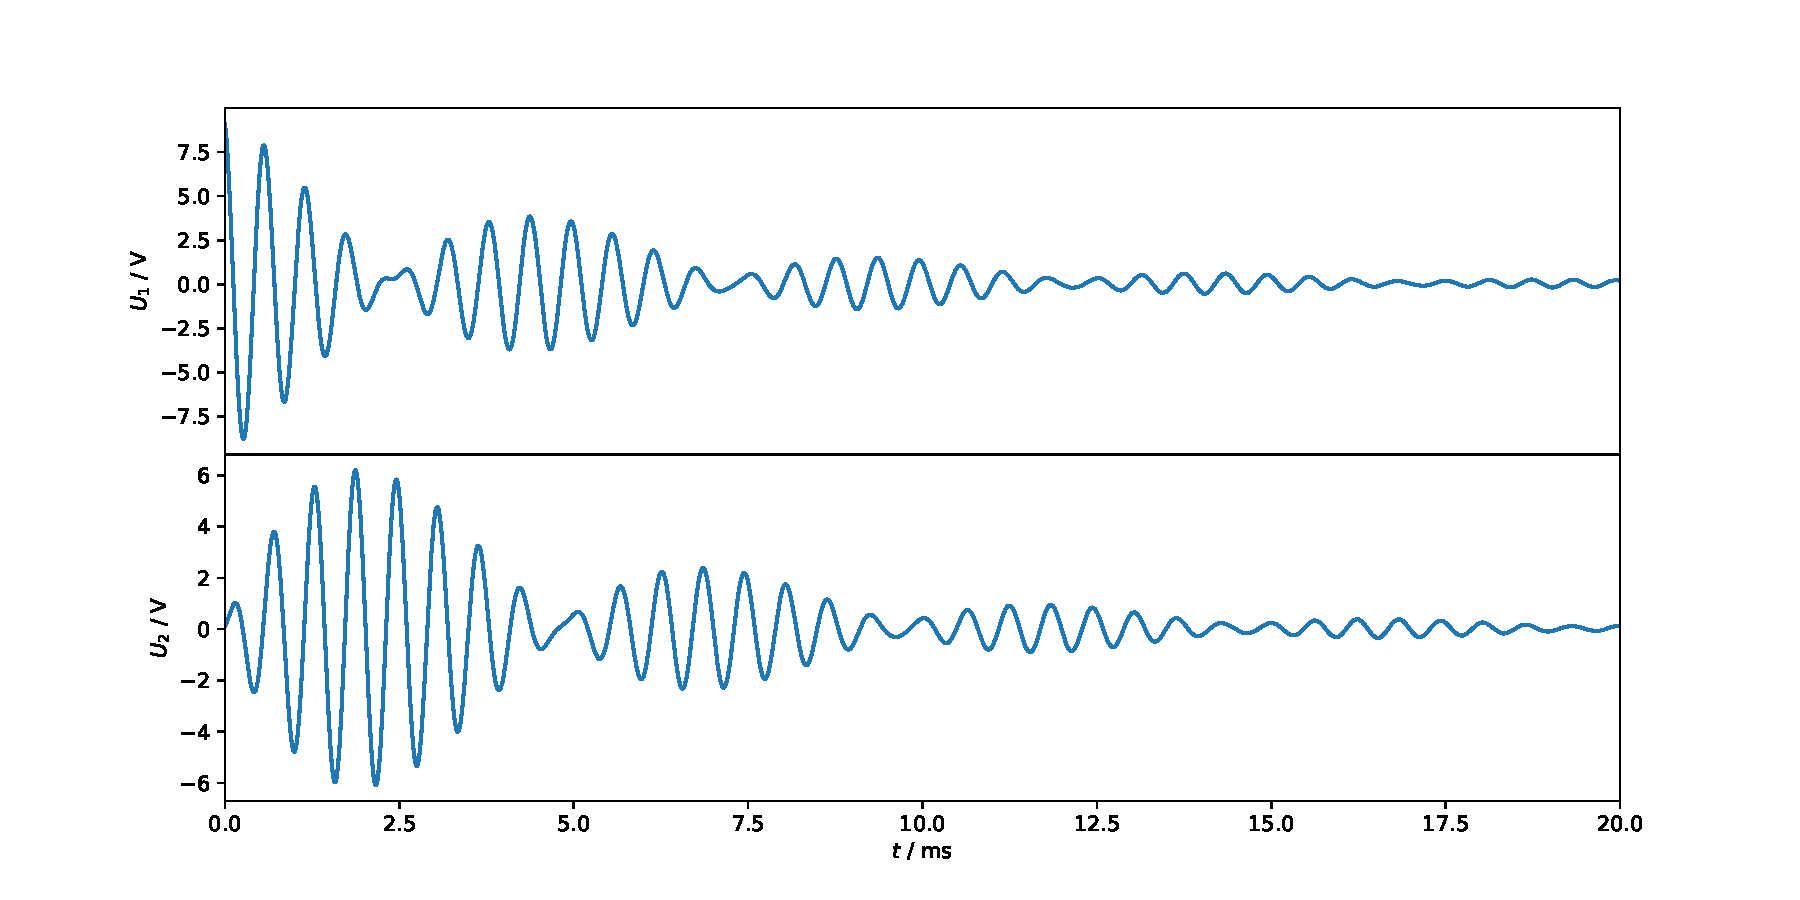
\includegraphics[width=\textwidth]{plots/schwebung_roh.pdf}
\caption{Rohdaten der Schwebung}
\label{abb:schwebung_roh}
\end{figure}

Da sich die Periodendauer der Schwebung bei den beiden anderen Schwebungen garnicht anhand der Schwebungsmaxima bestimmen lässt, wird ausschließlich eine Auswertung mittels FFT vorgenommen. Dabei ergeben sich die Frequenzen in Tabelle \ref{tab:freq_schweb} für die aufgezeichnete Spannung am ersten Kondensator.

\begin{table}[H]
\centering
\begin{tabular}{c|c|c}
Schwebung & $f_+$ / Hz & $f_-$ / Hz \\
\hline
1 & $1598.65 \pm 0.95$ & $1832.1 \pm 7.5$ \\
2 & $1639 \pm 11$ & $1727 \pm 23$ \\
3 & $631.8 \pm 6.9$ & $1094 \pm 19$
\end{tabular}
\caption{Frequenzen aus FFT}
\label{tab:freq_schweb}
\end{table}

Mithilfe der Frequenzen lassen sich nun die Kopplungsgrade der drei Konfigurationen berechnen. Es gilt
$$k = \frac{f_-^2 - f_+^2}{f_-^2 + f_+^2}.$$
Mittels Gaußscher Fehlerfortpflanzung lässt sich der Fehler auf $k$ zu
$$\sigma_k = \frac{4f_-f_+}{(f_-^2+f_+^2)^2} \sqrt{f_+^2 \sigma_{f_-}^2 + f_-^2 \sigma_{f_+}^2}$$
bestimmen. Es ergeben sich die Werte in Tabelle \ref{tab:kopplung}.

\begin{table}[H]
\centering
\begin{tabular}{c|c}
Schwebung & $k$ \\
\hline
1 & $0.1355 \pm 0.0041$ \\
2 & $0.0522 \pm 0.0146$ \\
3 & $0.4999 \pm 0.0155$
\end{tabular}
\caption{Berechnete Kopplungsgrade}
\label{tab:kopplung}
\end{table}


\subsubsection{Fazit}